% Created 2021-09-27 Mon 12:02
% Intended LaTeX compiler: xelatex
\documentclass[letterpaper]{article}
\usepackage{graphicx}
\usepackage{grffile}
\usepackage{longtable}
\usepackage{wrapfig}
\usepackage{rotating}
\usepackage[normalem]{ulem}
\usepackage{amsmath}
\usepackage{textcomp}
\usepackage{amssymb}
\usepackage{capt-of}
\usepackage{hyperref}
\setlength{\parindent}{0pt}
\usepackage[margin=1in]{geometry}
\usepackage{fontspec}
\usepackage{svg}
\usepackage{cancel}
\usepackage{indentfirst}
\setmainfont[ItalicFont = LiberationSans-Italic, BoldFont = LiberationSans-Bold, BoldItalicFont = LiberationSans-BoldItalic]{LiberationSans}
\newfontfamily\NHLight[ItalicFont = LiberationSansNarrow-Italic, BoldFont       = LiberationSansNarrow-Bold, BoldItalicFont = LiberationSansNarrow-BoldItalic]{LiberationSansNarrow}
\newcommand\textrmlf[1]{{\NHLight#1}}
\newcommand\textitlf[1]{{\NHLight\itshape#1}}
\let\textbflf\textrm
\newcommand\textulf[1]{{\NHLight\bfseries#1}}
\newcommand\textuitlf[1]{{\NHLight\bfseries\itshape#1}}
\usepackage{fancyhdr}
\pagestyle{fancy}
\usepackage{titlesec}
\usepackage{titling}
\makeatletter
\lhead{\textbf{\@title}}
\makeatother
\rhead{\textrmlf{Compiled} \today}
\lfoot{\theauthor\ \textbullet \ \textbf{2021-2022}}
\cfoot{}
\rfoot{\textrmlf{Page} \thepage}
\renewcommand{\tableofcontents}{}
\titleformat{\section} {\Large} {\textrmlf{\thesection} {|}} {0.3em} {\textbf}
\titleformat{\subsection} {\large} {\textrmlf{\thesubsection} {|}} {0.2em} {\textbf}
\titleformat{\subsubsection} {\large} {\textrmlf{\thesubsubsection} {|}} {0.1em} {\textbf}
\setlength{\parskip}{0.45em}
\renewcommand\maketitle{}
\author{Houjun Liu}
\date{\today}
\title{Guided Problem --- Particle Interactions, Coloumb's law}
\hypersetup{
 pdfauthor={Houjun Liu},
 pdftitle={Guided Problem --- Particle Interactions, Coloumb's law},
 pdfkeywords={},
 pdfsubject={},
 pdfcreator={Emacs 28.0.50 (Org mode 9.4.4)}, 
 pdflang={English}}
\begin{document}

\tableofcontents



\section{And now, a Guided Problem Solve}
\label{sec:org232d513}
\begin{figure}[htbp]
\centering
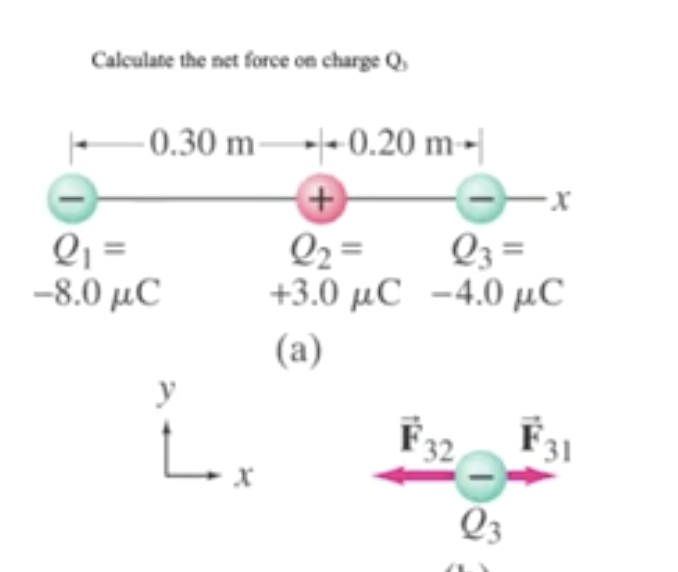
\includegraphics[width=.9\linewidth]{./2020PHYS201/Screen Shot 2020-08-24 at 8.06.36 PM.png}
\caption{Screen Shot 2020-08-24 at 8.06.36 PM.png}
\end{figure}

\textbf{Notice! This one is a little different because there are three
charges.}

We could see that, because of the fact that \(Q_2\) is closer to \(Q3\)
then \(Q1\) is and the two particles are pulling in different
directions, we could infer that \(||F_{32}||\) is larger then
\(||F_{31}||\). Because of this, we could find that \(Q_3\) will have a
net force "to the left" --- in \(F_{32}\)'s direction.

And, because of that, we know that \(Q_3\) will be accelerating towards
the left. But \textbf{Notice}!, whenever \(Q_3\) moves towards the left, the
distances between the particles changed, meaning the force acting upon
\(Q_3\) changes! Meaning, \(Q_3\)'s acceleration "to the left" is not
constant. Unfortunately, then, no equation of kinematics for us :(.
\end{document}
